
\section{Photometric properties}\label{sec:phot}

We studied the effect of dust obscuration on the colors of \euclid accessible galaxies in \textsc{Flares} using the UV continuum slope, $\rm \beta$.  \textcolor{red}{*** Not sure how to start this section *** want to discuss: selection of FUV (1500Å) and NUV (2500Å) for the analysis (middle of H and Y bands at z=6, though not accessible by H-band anymore after Z=7. -> need to supplement with spitzer or some such}

The luminosities were measured using two synthetic top-hat broadband filters; one for far ultraviolet (FUV) and one for near ultraviolet (NUV). The $\rm \beta$s were then measured using
\begin{equation}
\centering
    \mathrm{\beta = \frac{1}{log_{10}{\lambda^{FUV} / \lambda^{NUV}}} log_{10} \left ( \frac{L_{\nu}^{FUV}}{L_{\nu}^{NUV}} \right )  - 2  },
    \label{eqn:beta}
\end{equation}
\noindent
where $\rm L_{\nu}^{FUV}$ ($\rm L_{\nu}^{NUV}$) is the luminosity of the object for a top-hat filter centered at wavelength $\rm \lambda^{FUV} = 1500 $\AA  ($\rm \lambda^{NUV} = 2500 $\AA).

Figure \ref{fig:beta_summary} shows the rest-frame evolution of the mean UV continuum slope $\rm \beta$ as a function of $\rm H$-band flux for galaxies accessible to \euclid. We compare the effect of dust on $\rm \beta$ compared to intrinsic pure stellar and stellar + nebular emission cases. On average, adding nebular emission makes $\rm \beta$ redder (more positive) compared to the pure stellar case by $\rm {\sim}0.07$ $(\rm {\sim}0.1)$ at $\rm z=5$ $(\rm z=9)$. Adding dust further reddens $\rm \beta$ on average by $\rm {\sim}0.43$ $(\rm {\sim}0.46)$ at $\rm z=5$ $(\rm z=9)$. The flux relation of the dust obscured UV continuum slope flattens for galaxies accessible to \euclid \: ($\rm H < 26$). \textcolor{red}{*** ADD MORE TO THIS ***} Figure \ref{fig:beta_all} shows more detailed account of $\rm \beta$ evolution for all the redshifts considered ($\rm z = [5, 10]$). The mean $\rm \beta$ is roughly the same ($\rm \Bar{\beta} \approx -1.9 $) at all considered redshifts for \euclid \: accessible galaxies.


\begin{figure}
	\centering
	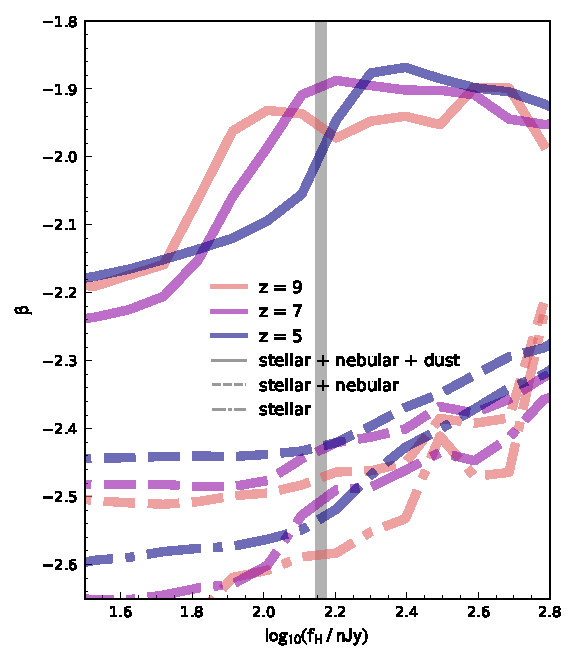
\includegraphics[width=0.5\textwidth]{./figures/beta/beta_summary.pdf}
	\caption{Median UV continuum slope ($\beta$) as a function of observed $\rm H$-band flux. The vertical line shows the $\rm H = 26$ limit. The relation between $\rm \beta$ and brightness flattens out for galaxies brighter than $\rm H \sim 26$. \label{fig:beta_summary}}
\end{figure}


\begin{figure}
	\centering
	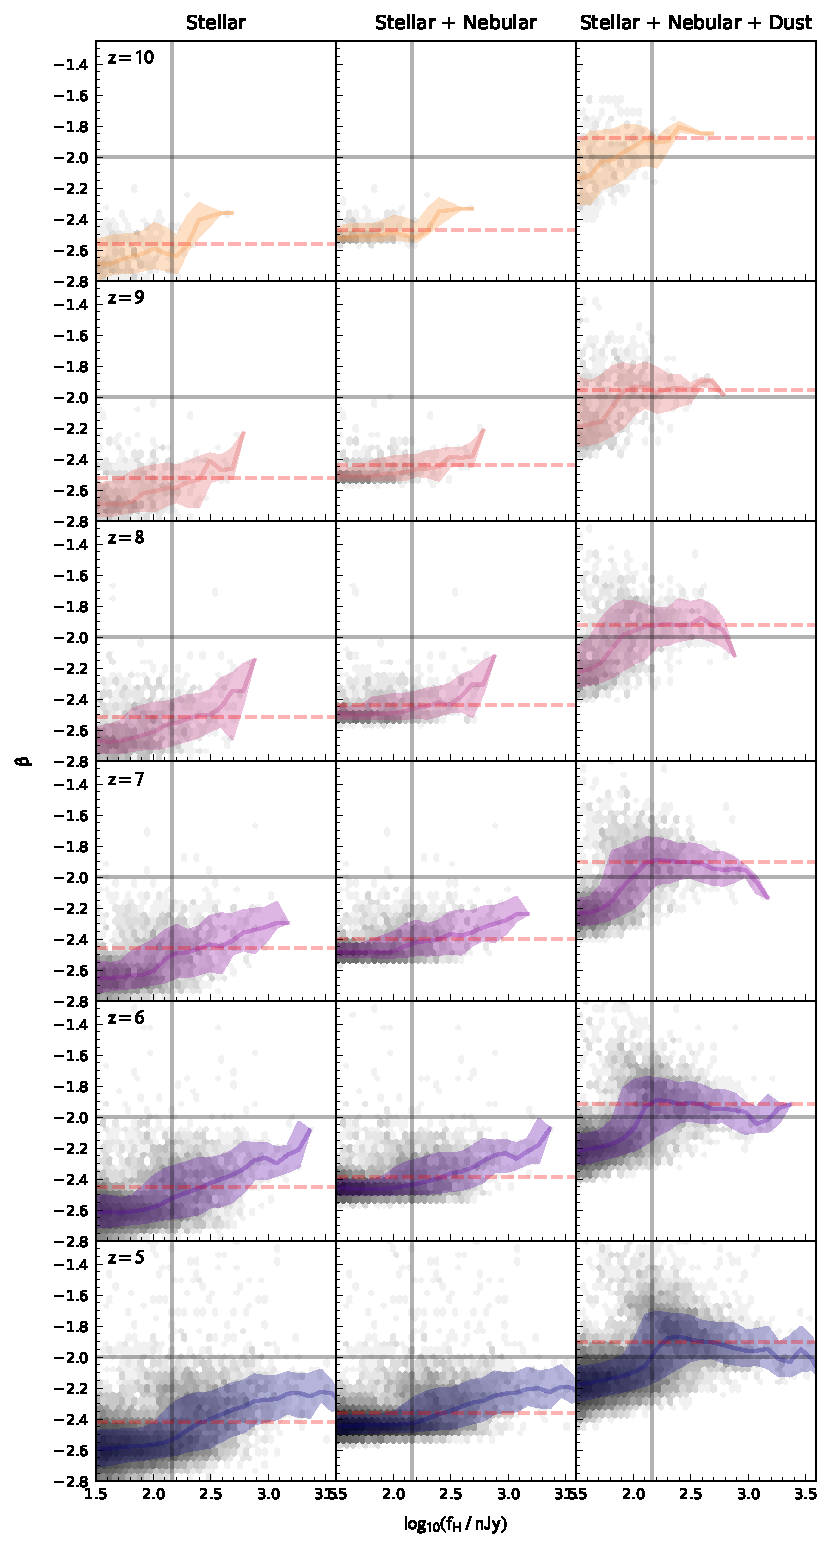
\includegraphics[width=0.5\textwidth]{./figures/beta/beta_all}
	\caption{UV continuum slope $\beta$ vs. $\rm H$-band flux for all considered EoR redshifts. The solid line shows the median of the $\rm \beta$ distribution and the shaded region shows the corresponding 84\% - 16\% range. The vertical lines show the $\rm H = 26$ limit, horizontal black line shows $\rm \beta = -2$ (to guide the eye) and the horizontal red dashed line shows median $\rm \beta$ for galaxies accessible to \euclid. \label{fig:beta_all}}
\end{figure}